\section{Задача классификации}

\subsection{CatBoost}

Самый простой среди мощных и самый мощный среди простых -- CatBoost~\cite{CatboostDocs}. Эта библиотека, которая решает задачу классификации. Она основана на градиентном бустинге, надстройкой над решающими деревьями. Как оно работает внутри -- тема другой работы, здесь мы рассмотрим ее применение.

\subsection{Данные}

\subsubsection{Датасет}

По индикатором, которые мы выбрали, нужно построить датасет. Мы его устроили так:

\begin{enumerate}

    \item Посчитали значения индикаторов по каждой из сторон за последние \texttt{n/c, 2n/c, ..., n} секунд.
    
    \item Распарсили так, что по столбцам данные за промежутки \texttt{[0, n/c], [n/c, 2n/c], ..., [(c - 1)n/c, n]} секунд.
    
    \item Параметры выбрали такие: \texttt{n = 60, c = 10}.
    
    \item В качестве вектора ответов у нас единица, если рынок отклонился более, чем на $\Delta$ вверх, -1, если вниз, и 0 иначе. $\Delta$ экспериментально выбрали как 5 * \texttt{commision, commision = 0.02\%}.
    
\end{enumerate}

\subsubsection{Парсинг}

Код:
\begin{enumerate}
\item \href{https://github.com/dexety/dex-trading-system/blob/main/research/lp-0004-trades-volume/parse/parse_trades_data.py}{Парсер}. 
\item \href{https://github.com/dexety/dex-trading-system/blob/main/utils/buy_sell_queue.py}{Очередь на минимумы/максимумы}.
\item \href{https://github.com/dexety/dex-trading-system/blob/main/utils/indicators.py}{Индикаторы}.
\end{enumerate}


Парсер устроен так:

\begin{enumerate}

\item У нас есть две очереди на минимумы/максимумы. Мы написали свою реализацию \texttt{BuySellSqueue}. Часть операций, которые поддерживает эта очередь:
\begin{enumerate}
    \item \texttt{pop\_front}
    \item \texttt{push\_back}
    \item \texttt{get\_side\_queue\_max\_price}
    \item \texttt{get\_side\_queue\_min\_price}
\end{enumerate}

\item В каждый момент времени в первой очереди у нас все трейды за последний 60 секунд, а во второй за последующие 30. Эти параметры можно настраивать. 
\item После чтения очередного трейда мы обновляем очереди и с какой-то вероятностью пересчитываем индикаторы. Делаем это не всегда, потому что количество трейдов огромное, и построить датасет по всем сделкам невозможно из-за ограничений по памяти.
    
\end{enumerate}

\subsection{Индикаторы}

Класс \href{https://github.com/dexety/dex-trading-system/blob/ca0370d602f2dfa05262b9b8574002f965ac1502/utils/indicators.py#L5}{\texttt{Indicators}} содержит функции, заполняющие значения фичей и столбца таргета: \texttt{fill\_features\_values} и \texttt{fill\_target\_values}.

\subsubsection{\texttt{fill\_target\_values}}
\href{https://github.com/dexety/dex-trading-system/blob/ca0370d602f2dfa05262b9b8574002f965ac1502/utils/indicators.py#L15}{Функция в репозитории}

Функция принимает словарь для заполнения значений, две очереди трейдов и параметры ордеров \texttt{stop\_profit} и \texttt{stop\_loss}. Функция считает, исполнились бы эти ордеры и выставляет соответствующее значение в словарь для заполнения.

\subsubsection{\texttt{fill\_features\_values}}
\href{https://github.com/dexety/dex-trading-system/blob/ca0370d602f2dfa05262b9b8574002f965ac1502/utils/indicators.py#L48}{Функция в репозитории}

\begin{designation}
Окно длины $t$ -- очередь, в которой есть все трэйды, случившиеся не больше чем за $t$ секунд до какого-то момента. Обозначаем как \textit{window}.
\end{designation}

\begin{designation}
    \texttt{window[i]} -- i-ый элементы в окне.
\end{designation}
\begin{designation}
    \texttt{window[i].price} и \texttt{window[i].volume} -- цена и объем i-й сделки в окне соответсвенно.
\end{designation}

Функция принимает словарь для заполнения, окно трэйдов, и два списка вариантов числовых параметров фичей $n$ и $t$. За $n$ всегда будем обозначать количество сделок в окне. Функция заполняет словарь значениями фичей, которые представлены ниже:

\begin{enumerate}
    \item \texttt{seconds\_since\_midnight} -- количество секунд с начала дня.
    \item \texttt{seconds\_since\_n\_trades\_ago} -- количество секунд, прошедших с первого трэйда в окне из $n$ последних трэйдов.
    
    \textbf{Псевдо-формула:} \texttt{(window.end\_time - window[-n].time).to\_seconds()}

    \item \texttt{WI\_exp\_moving\_average} -- экспоненциальное среднее в окне длины $t$. 
    
    \textbf{Псевдо-формула:} \texttt{$\alpha$ (window[-1].price + $(1 - \alpha)$ window[-2].price + \dots + $(1 - \alpha)^{n - 1}$ window[-n].price)}

    \item \texttt{WI\_weighted\_moving\_average} -- взвешанное среднее в окне длины $t$.

    \textbf{Псевдо-формула:} $\frac{\sum\limits_{i=0}^{n} \texttt{window[i].price} \; \cdot \; \texttt{window[i].volume}}{\sum\limits_{i=0}^{n}\texttt{window[i].size}}$

    \item \texttt{WI\_trade\_amount} -- количество сделок в окне длины $t$.

    \textbf{Псевдо-формула:} n

    \item \texttt{WI\_trade\_volume} -- суммарный объем сделок в окне длины $t$.

    \textbf{Псевдо-формула:} $\sum\limits_{i=0}^{n}\texttt{window[i].volume}$

    \item \texttt{WI\_open\_close\_diff} -- \textbf{частное} между ценой закрытия и ценой открытия в окне длины $t$.

    \textbf{Псевдо-формула:} \texttt{window[-1].price / window[0].price}

    \item \texttt{WI\_stochastic\_oscillator} -- стохастический осцилятор.

    \textbf{Псевдо-формула:} $\frac{\texttt{CUR} - \texttt{MIN}}{\texttt{MAX} - \texttt{MIN}}$, где \texttt{CUR} - цена последней сделки, а \texttt{MIN} и \texttt{MAX} - наименьшая и наибольшая цена сделки соответственно в окне длины $t$.

\end{enumerate}

Вторая фича зависит от значения $n$ и от направления трэйдов в окне, поэтому для каждой комбинации направления и параметра $n$ в таблице будет свой столбец.

Последние 5 фичей зависят от $t$ и от направления трэйдов в окне, поэтому для каждой комбинации направления, параметра $t$ и фичи в таблице будет свой столбец.

В послдедствии мы решили еще дополнительно делить все скользящие средние на среднее арифметическое цен всех сделок в окне. 

\textbf{Псевдо-формула:} $\texttt{WI\_moving\_average} \; \cdot \; \frac{n}{\sum\limits_{i=0}^{n - 1} window[i].price}$ 

Это сделано для того, чтобы при глобальном изменении стоимости валюты модель продолжала работать.


\subsection{Использование CatBoost}

\subsubsection{Fit-Predict}

\begin{verbatim}
params = {
    'iterations': 300,
    'l2_leaf_reg': int(best['l2_leaf_reg']),
    'learning_rate': best['learning_rate'],
    'custom_loss': [metrics.Accuracy()],
    'eval_metric': metrics.Accuracy(),
    'random_seed': 42,
    'logging_level': 'Silent',
    'loss_function': 'Logloss',
}
train_pool = Pool(X_train, y_train)
validate_pool = Pool(X_validation, y_validation)
model = CatBoostClassifier(**params)
model.fit(
    train_pool,
    eval_set=validate_pool,
    plot=True,
)
predictions = model.predict(X_test)
predictions = predictions.reshape(predictions.shape[0], 1)
predictions_probs = model.predict_proba(X_test)
\end{verbatim}

\subsubsection{Автоподбор гипер-параметров}

\begin{verbatim}

def hyperopt_objective(params):
    model = CatBoostClassifier(
        l2_leaf_reg=int(params['l2_leaf_reg']),
        learning_rate=params['learning_rate'],
        iterations=300,
        eval_metric=metrics.Accuracy(),
        random_seed=126,
        verbose=False,
        loss_function=metrics.Logloss(),
    )
    cv_data = cv(
        Pool(X, y),
        model.get_params(),
        fold_count=5,
        shuffle=True,
        logging_level='Silent',
    )
    best_accuracy = np.max(cv_data['test-Accuracy-mean'])
    return 1 - best_accuracy

params_space = {
    'l2_leaf_reg': hyperopt.hp.qloguniform('l2_leaf_reg', 0, 2, 1),
    'learning_rate': hyperopt.hp.uniform('learning_rate', 1e-3, 5e-1),
}
trials = hyperopt.Trials()
best = hyperopt.fmin(
    hyperopt_objective,
    space=params_space,
    algo=hyperopt.tpe.suggest,
    max_evals=50,
    trials=trials,
    rstate=RandomState(42)
)

\end{verbatim}

\subsection{FPR/FNR}

\definition \textbf{False Positive/Negative Ratio} -- отношения ложно-положительных/ложно-отрицательных предсказаний ко всем отрицатльным/положительным.

\designation FPR/FNR

Мы хотим оптимизировать лучше FPR, чем FNR, потому что в первом случае мы теряем деньгии, а во втором не получаем.

Параметр $\Delta$ подобран так, что

$$\texttt{FPR} = \frac{\texttt{false positive}}{\texttt{total negative num}} = 0.010005175090564086$$

$$\texttt{FnR} = \frac{\texttt{false negative}}{\texttt{total positive num}} = 0.8827444956477215$$

Эксперимент показал, что такие значения достигаются при плече принятия решений $\omega = 34\%$. То есть если модель предсказывает $\pm 1$ с такой вероятностью или больше, то мы считаем, что ее прогноз верный. Причем мы не хотим оказаться в ситуации, когда модель выдает $P(1) = 45\%$, $P(-1) = 45.1\%$ , порог в $34\%$ пройден, значит надо выбирать -1. Но мы хотим выбрать -1 только тогда, когда $P(-1) \geqslant \omega \cap P(-1) > (P(1) + \varepsilon) \cap P(-1) > (P(0) + \varepsilon)$. Эксперимент выдал, что $\varepsilon = 1\%$ оптимальнее всего.

\subsection{Важность индикаторов}
После того, как мы обучили модель, можно посмотреть самые важные индикаторы, которые выбрал \texttt{CatBoost}. Сделать это можно командой

\begin{verbatim}
feature_importances = model.get_feature_importance(train_pool)
feature_names = X_train.columns
for score, name in sorted(zip(feature_importances, feature_names), reverse=True):
    print('{}: {}'.format(name, score))
\end{verbatim}

Топ-15 индикаторов оказались:
\begin{enumerate}
\item \texttt{open-close-diff-SELL-60-sec}
\item \texttt{stochastic-oscillator-BUY-600-sec}
\item \texttt{open-close-diff-SELL-600-sec}
\item \texttt{open-close-diff-BUY-60-sec}
\item \texttt{stochastic-oscillator-SELL-600-sec}
\item \texttt{open-close-diff-BUY-600-sec}
\item \texttt{open-close-diff-BUY-30-sec}
\item \texttt{open-close-diff-SELL-30-sec}
\item \texttt{seconds-since-1000-trades-ago-BUY}
\item \texttt{seconds-since-midnight}
\item \texttt{seconds-since-10-trades-ago-BUY}
\item \texttt{seconds-since-100-trades-ago-BUY}
\item \texttt{seconds-since-50-trades-ago-BUY}
\item \texttt{trade-amount-BUY-60-sec}
\item \texttt{stochastic-oscillator-BUY-60-sec}
\end{enumerate}

\subsection{Распределение индикаторов}

Чтобы понять, насколько хорошо модель может обучиться, надо посмотреть на распределение индикаторов по разным таргетам. Хочется, чтобы как можно большая часть распределение разных таргетов не пересекалась, потому что тогда алгоритм решающих деревьев будет справляться лучше всего.

Посмотрим на распределение всех фичей, и поближе на \texttt{seconds-since-50-trades-ago-BUY} и \\ \texttt{open-close-diff-SELL-30-sec}

\begin{figure}[H]
\centering
\subfloat[Распределение фичей]{
    \includegraphics[width=0.9\linewidth]{img/dist.png}
    }
\end{figure}


\begin{figure}[H]
\centering
\subfloat[seconds-since-50-trades-ago-BUY]{
    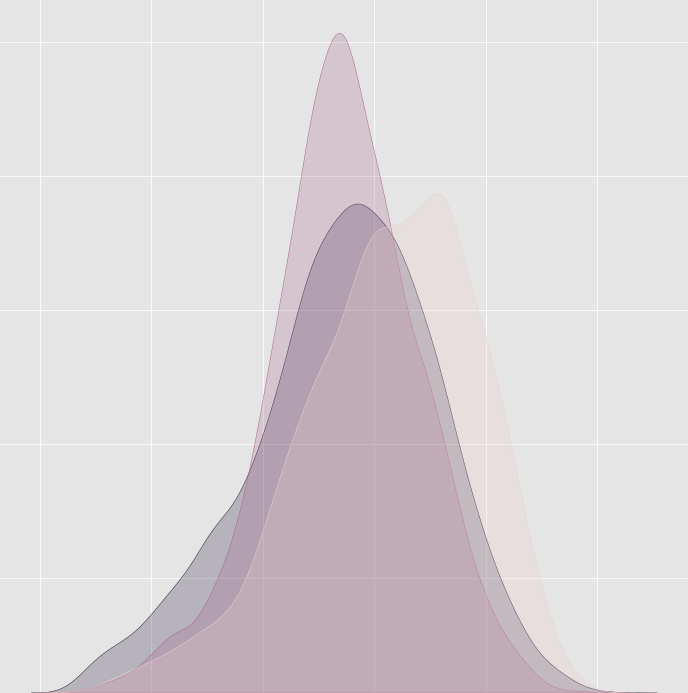
\includegraphics[width=0.35\linewidth]{img/seconds-since-50-trades-ago-BUY.png}
    }
\subfloat[open-close-diff-SELL-30-sec]{
    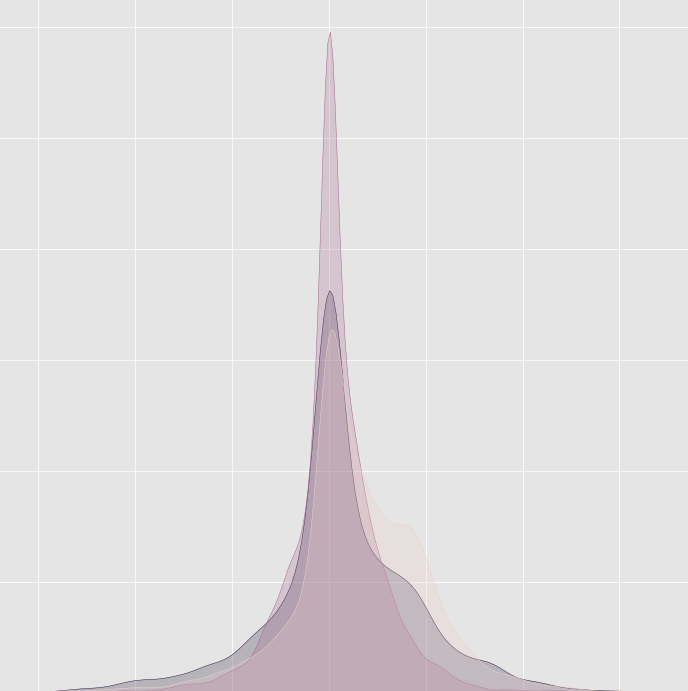
\includegraphics[width=0.35\linewidth]{img/open-close-diff-SELL-30-sec.png}
    }
\end{figure}

Видим, что оба распределения такие, что почти невозможно отличить один таргет от другого, только на \href{fig:trades_ago} можно немного отличить таргет $-1$, который бежевого цвета. Поэтому ждать, что модель у нас получится хорошая не приходится.



\subsection{Результат}
При таких параметрах получается, что моделька в $9.78\%$ случаев с вероятностью $69.63\%$ правильно предсказывает скачок рынка. То есть из всех скачков она ловит только $9.78\%$. И среди них с вероятностью $69.63\%$ угадывает, куда пойдет рынок.

Однако если учитывать комиссию биржи, то мы будем играть в минус.
